\documentclass[12pt,a4paper]{article}
\usepackage{cmap} % Makes the PDF copiable. See http://tex.stackexchange.com/a/64198/25761
\usepackage[T1]{fontenc}
\usepackage[brazil]{babel}
\usepackage[utf8]{inputenc}
\usepackage{amsmath}
\usepackage{amsfonts}
\usepackage{amssymb}
\usepackage{amsthm}
\usepackage[usenames,svgnames,dvipsnames]{xcolor}
\usepackage{hyperref}
\usepackage{multicol}
\usepackage{graphicx}
\usepackage[margin=2cm]{geometry}

\hypersetup{
    colorlinks = true,
    allcolors = {blue}
}

% TODO: Consider using exsheets
% http://linorg.usp.br/CTAN/macros/latex/contrib/exsheets/exsheets_en.pdf
%
% http://ctan.org/tex-archive/macros/latex/contrib/exercise/
% Options: answerdelayed,lastexercise,noanswer
\usepackage[answerdelayed,lastexercise]{exercise}

\addto\captionsbrazil{%
\def\listexercisename{Lista de exerc\'icios}%
\def\ExerciseName{Exerc\'icio}%
\def\AnswerName{Solu\c{c}\~ao do exerc\'icio}%
\def\ExerciseListName{Ex.}%
\def\AnswerListName{Solu\c{c}\~ao}%
\def\ExePartName{Parte}%
\def\ArticleOf{de\ }%
}

\renewcommand{\ExerciseHeaderTitle}{(\ExerciseTitle)\ }
\renewcommand{\ExerciseListHeader}{%\ExerciseHeaderDifficulty%
\textbf{%\ExerciseListName\
\ExerciseHeaderNB.\ %
%\ --- \
\ExerciseHeaderTitle}%
%\ExerciseHeaderOrigin
\ignorespaces}
\renewcommand{\AnswerListHeader}{\textbf{\ExerciseHeaderNB.\ (\AnswerListName)\ }}

\newcommand*\diff{\mathop{}\!\mathrm{d}}
\newcommand*\sen{\operatorname{sen}}

\renewcommand{\theenumi}{\alph{enumi}}
\renewcommand\labelenumi{(\theenumi) }

\newcommand*\tipo{Prova III}
\newcommand*\turma{PRO112-02U}
\newcommand*\disciplina{CDI2001}
\newcommand*\eu{Helder G. G. de Lima}
\newcommand*\data{06/12/2024}

\author{\eu}
\title{\tipo - \disciplina}
\date{\data}

\begin{document}
\thispagestyle{empty}
\newgeometry{margin=2cm,bottom=0.5cm}
\begin{center}

\includegraphics[width=9.0cm]{marca} \\
\textbf{\tipo\ (\disciplina / \turma)} \\
Prof. \eu\footnote{
Este é um material de acesso livre distribuído sob os termos da licença \href{https://creativecommons.org/licenses/by-sa/4.0/deed.pt_BR}{Creative Commons BY-SA 4.0}}
\end{center}

\noindent Nome do(a) aluno(a): \underline{\hspace{9,7cm}} Data: \underline{\data}

\begin{center}\fbox{
\begin{minipage}{14cm}

{\footnotesize
\begin{itemize}
\renewcommand{\theenumi}{\Roman{enumi}}
\item Identifique-se em todas as folhas.
\item Não é permitido o uso de calculadora.
\item Mantenha o celular e os demais equipamentos eletrônicos desligados durante a prova.
\item Justifique cada resposta com cálculos ou argumentos baseados na teoria estudada.
\item Resolva $4$ das $5$ questões (deixe claro que questão não deverá ser corrigida).
\end{itemize}
}

\end{minipage}
}
\end{center}

\begin{ExerciseList}
\Exercise[title={2,5}] Determine todos os pontos em que a função a seguir é contínua:
\[
f(x, y) = 
\begin{cases}
    \frac{(2x + y)^2}{4x^2 + y^2}, & \text{se } (x, y) \neq (0, 0), \\
    1, & \text{se } (x, y) = (0, 0).
\end{cases}
\]

\Answer Há dois casos a considerar:
\begin{enumerate}
\item A função \(\boxed{\text{é contínua em todos os pontos } (x, y) \neq (0, 0)}\), pois é o quociente de funções contínuas com denominador não nulo. 
\item Entretanto, ela \(\boxed{\text{não é contínua no ponto } (x, y) = (0, 0)}\), já que não tem limite nesse ponto. De fato, limites diferentes são obtidos ao considerar diferentes caminhos. Por exemplo,
\begin{itemize}
\item Pelo caminho $C_1 = \{(x, y)\mid x = 0 \} = \{(0, y)\mid y \in \mathbb{R} \}$, obtemos:
\[
\lim_{(x, y) \xrightarrow[C_1]{} (0, 0)} \frac{(2x + y)^2}{4x^2 + y^2}
  = \lim_{y\to 0} \frac{(2\cdot 0 + y)^2}{4\cdot 0^2 + y^2}
  = \lim_{y\to 0} \frac{y^2}{y^2}
  = \lim_{y\to 0} 1
  = 1 = f(0, 0).
\]
\item Pelo caminho $C_2 = \{(x, y)\mid y = -2x \} = \{(x, -2x)\mid x \in \mathbb{R} \}$, obtemos:
\[
\lim_{(x, y) \xrightarrow[C_2]{} (0, 0)} \frac{(2x + y)^2}{4x^2 + y^2}
  = \lim_{x\to 0} \frac{(2x + (-2x))^2}{4x^2 + (-2x)^2}
  = \lim_{x\to 0} \frac{0^2}{4x^2+4x^2}
  = \lim_{x\to 0} 0
  = 0 \neq 1.
\]
\item Em geral, por um caminho $C_3 = \{(x, y)\mid y = mx \} = \{(x, mx)\mid x \in \mathbb{R} \}$, obtemos:
\begin{align*}
\lim_{(x, y) \xrightarrow[C_3]{} (0, 0)} \frac{(2x + y)^2}{4x^2 + y^2}
& = \lim_{x\to 0} \frac{(2x + (mx))^2}{4x^2 + (mx)^2}
  = \lim_{x\to 0} \frac{4x^2 + 4mx^2 + m^2x^2}{4x^2 + m^2x^2} \\
& = \lim_{x\to 0} \frac{x^2(4 + 4m + m^2)}{x^2(4 + m^2)}
  = \lim_{x\to 0} \frac{4 + 4m + m^2}{4 + m^2}
  = \frac{4 + 4m + m^2}{4 + m^2}.
\end{align*}
\end{itemize}
\end{enumerate}

\begin{center}
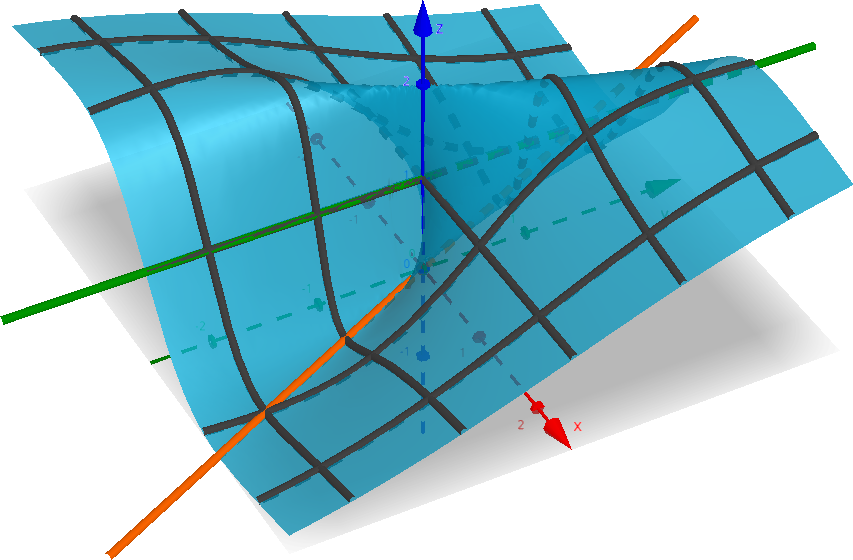
\includegraphics[width=0.5\textwidth]{img/continuidade.png}
\end{center}


\Exercise[title={2,5}] Obtenha a equação do plano tangente ao gráfico da função \(f(x, y) = (y^2 + 1)x e^x\) no ponto \(P = (0, -1, f(0, -1))\).

\Answer Calculando \(f(0, -1)\), temos:
\[
f(0, -1) = ((-1)^2 + 1) \cdot 0 \cdot e^0 = 0.
\]
As derivadas parciais são:
\[
\frac{\partial f}{\partial x}(x, y)
= \frac{\partial}{\partial x} \left[(y^2 + 1)x e^x \right]
= (y^2 + 1) \frac{\partial}{\partial x} \left[x e^x \right]
= (y^2 + 1)\left(e^x + x e^x\right)
= (y^2 + 1)e^x(x + 1),
\]
e
\[
\frac{\partial f}{\partial y}(x, y)
= \frac{\partial}{\partial y} \left[(y^2 + 1)x e^x \right]
= \frac{\partial}{\partial y} \left[(y^2 + 1)\right] \cdot x e^x
= 2y x e^x.
\]
Calculando as derivadas parciais em \((0, -1)\), obtemos:
\[
\frac{\partial f}{\partial x}(0, -1) = ((-1)^2 + 1)e^0(0 + 1) = 2, \quad
\frac{\partial f}{\partial y}(0, -1) = 2 \cdot (-1) \cdot 0 \cdot e^0 = 0.
\]
Portanto, a equação do plano tangente é:
\[
z - 0 = 2(x - 0) + 0(y - (-1)),
\]
ou seja, \(\boxed{z = 2x}\).

\begin{center}
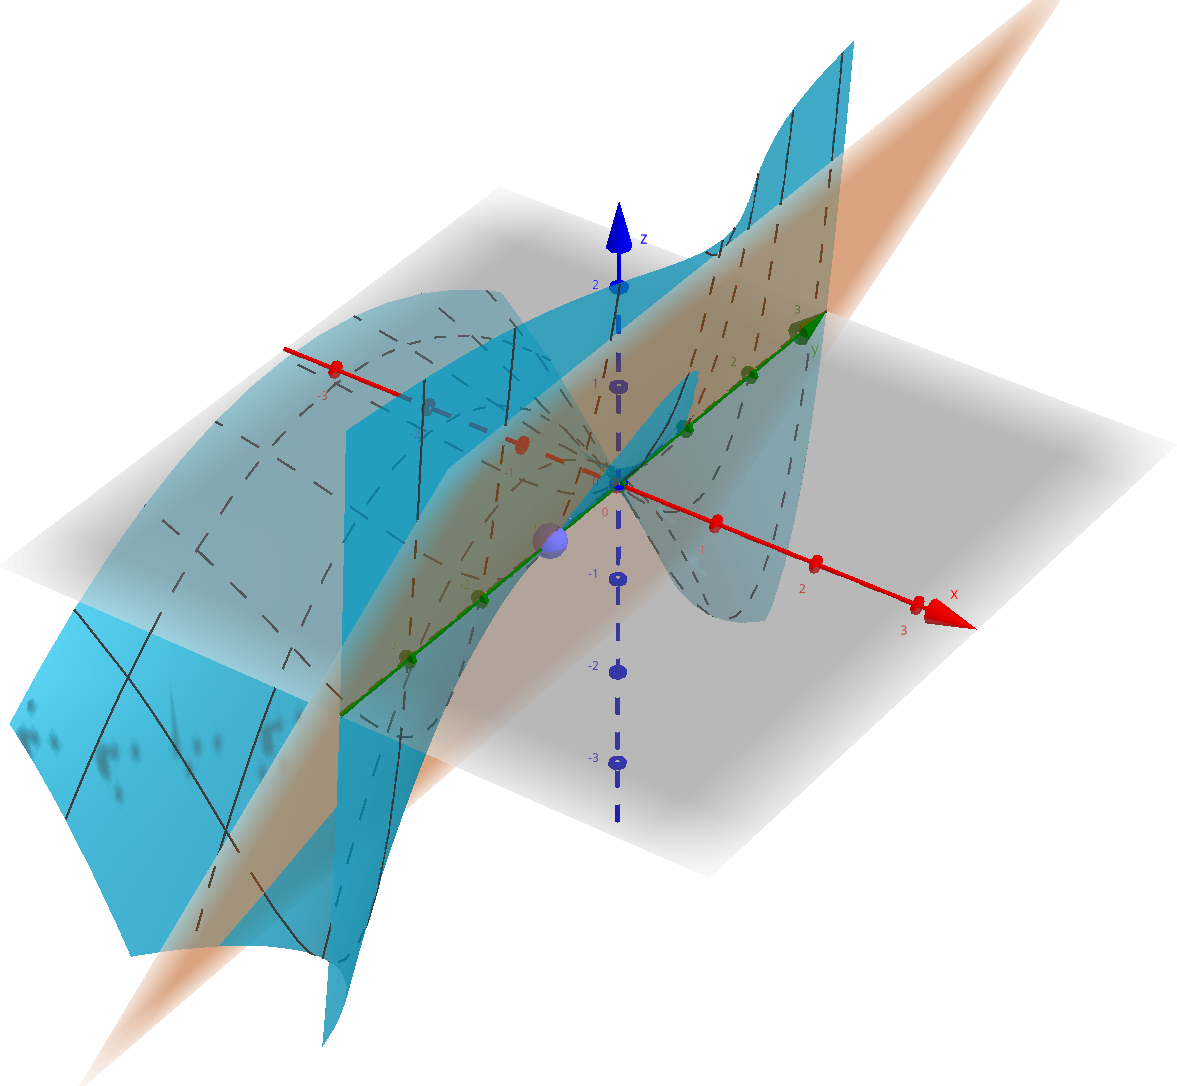
\includegraphics[width=0.5\textwidth]{img/plano-tangente.png}
\end{center}


\Exercise[title={2,5}] Classifique, se possível, os pontos críticos da função \(g(x, y) = 2y^2 - x^2 - y^4\).

\Answer As derivadas parciais de primeira ordem são:
\[
\frac{\partial g}{\partial x}(x, y) = -2x, \quad \frac{\partial g}{\partial y}(x, y) = 4y - 4y^3.
\]
Em um ponto crítico $(x, y)$, devemos ter \(\frac{\partial g}{\partial x}(x, y) = 0\) e \(\frac{\partial g}{\partial y}(x, y) = 0\). Neste caso,
\[
\frac{\partial g}{\partial x}(x, y) = 0 \implies x = 0, \quad
\frac{\partial g}{\partial y}(x, y) = 0 \implies 4y(1 - y^2) = 0 \implies y = 0 \text{ ou } y = \pm 1.
\]
Assim, os pontos críticos são \((0, 0)\), \((0, 1)\) e \((0, -1)\).

As derivadas de segunda ordem são:
\[
\frac{\partial^2 g}{\partial x^2}(x, y) = -2,
\quad
\frac{\partial^2 g}{\partial y^2}(x, y) = 4 - 12y^2,
\quad
\frac{\partial^2 g}{\partial x \partial y}(x, y) = 0.
\]
O determinante da matriz Hessiana é:
\[
H
= H(x, y)
= \begin{vmatrix}
    \frac{\partial^2 g}{\partial x^2}(x, y) & \frac{\partial^2 g}{\partial x \partial y}(x, y) \\
    \frac{\partial^2 g}{\partial y \partial x}(x, y) & \frac{\partial^2 g}{\partial y^2}(x, y)
\end{vmatrix}
= \begin{vmatrix}
    -2 & 0 \\
    0 & 4 - 12y^2
\end{vmatrix}
= (-2)(4 - 12y^2)
= -8 + 24y^2.
\]
Podemos então classificar os pontos críticos:
\begin{itemize}
    \item Em \((0, 0)\): \(H = -8 < 0\), então \(\boxed{(0, 0) \text{ é um ponto de sela}}\).
    \item Em \((0, 1)\) e \((0, -1)\): \(H = 16 > 0\) e \(\frac{\partial^2 g}{\partial x^2} < 0\), então \(\boxed{(0, \pm 1) \text{ são pontos de máximo locais}}\).
\end{itemize}

\begin{center}
\includegraphics[width=0.6\textwidth]{img/pontos-críticos.png}
\end{center}


\Exercise[title={2,5}]
Seja \(D\) a região entre as circunferências \(x^2 + y^2 = 9\) e \(x^2 + y^2 = 25\). Utilize coordenadas polares para calcular a integral dupla
\[
\iint_{D} \frac{1}{\sqrt{x^2 + y^2}} \diff{A}.
\]
\Answer Em coordenadas polares:
\[
x = r\cos(\theta), \quad y = r\sen(\theta), \quad x^2 + y^2 = r^2.
\]
Logo:
\begin{align*}
    \iint_{D} \frac{1}{\sqrt{x^2 + y^2}} \diff{A}
    & = \int_{0}^{2\pi} \int_{3}^{5} \frac{1}{\sqrt{r^2}} |r| \diff{r} \diff{\theta}
    = \int_{0}^{2\pi} \int_{3}^{5} \frac{1}{|r|} |r|\diff{r} \diff{\theta}
    = \int_{0}^{2\pi} \int_{3}^{5} 1\diff{r} \diff{\theta} \\
    & = \int_{0}^{2\pi} [r]_{3}^{5} \diff{\theta}
    = \int_{0}^{2\pi} 2 \diff{\theta}
    = 2[\theta]_{0}^{2\pi}
    = 2(2\pi - 0)
    = 4\pi.
\end{align*}
Portanto, \(\boxed{4\pi}\).

\begin{center}
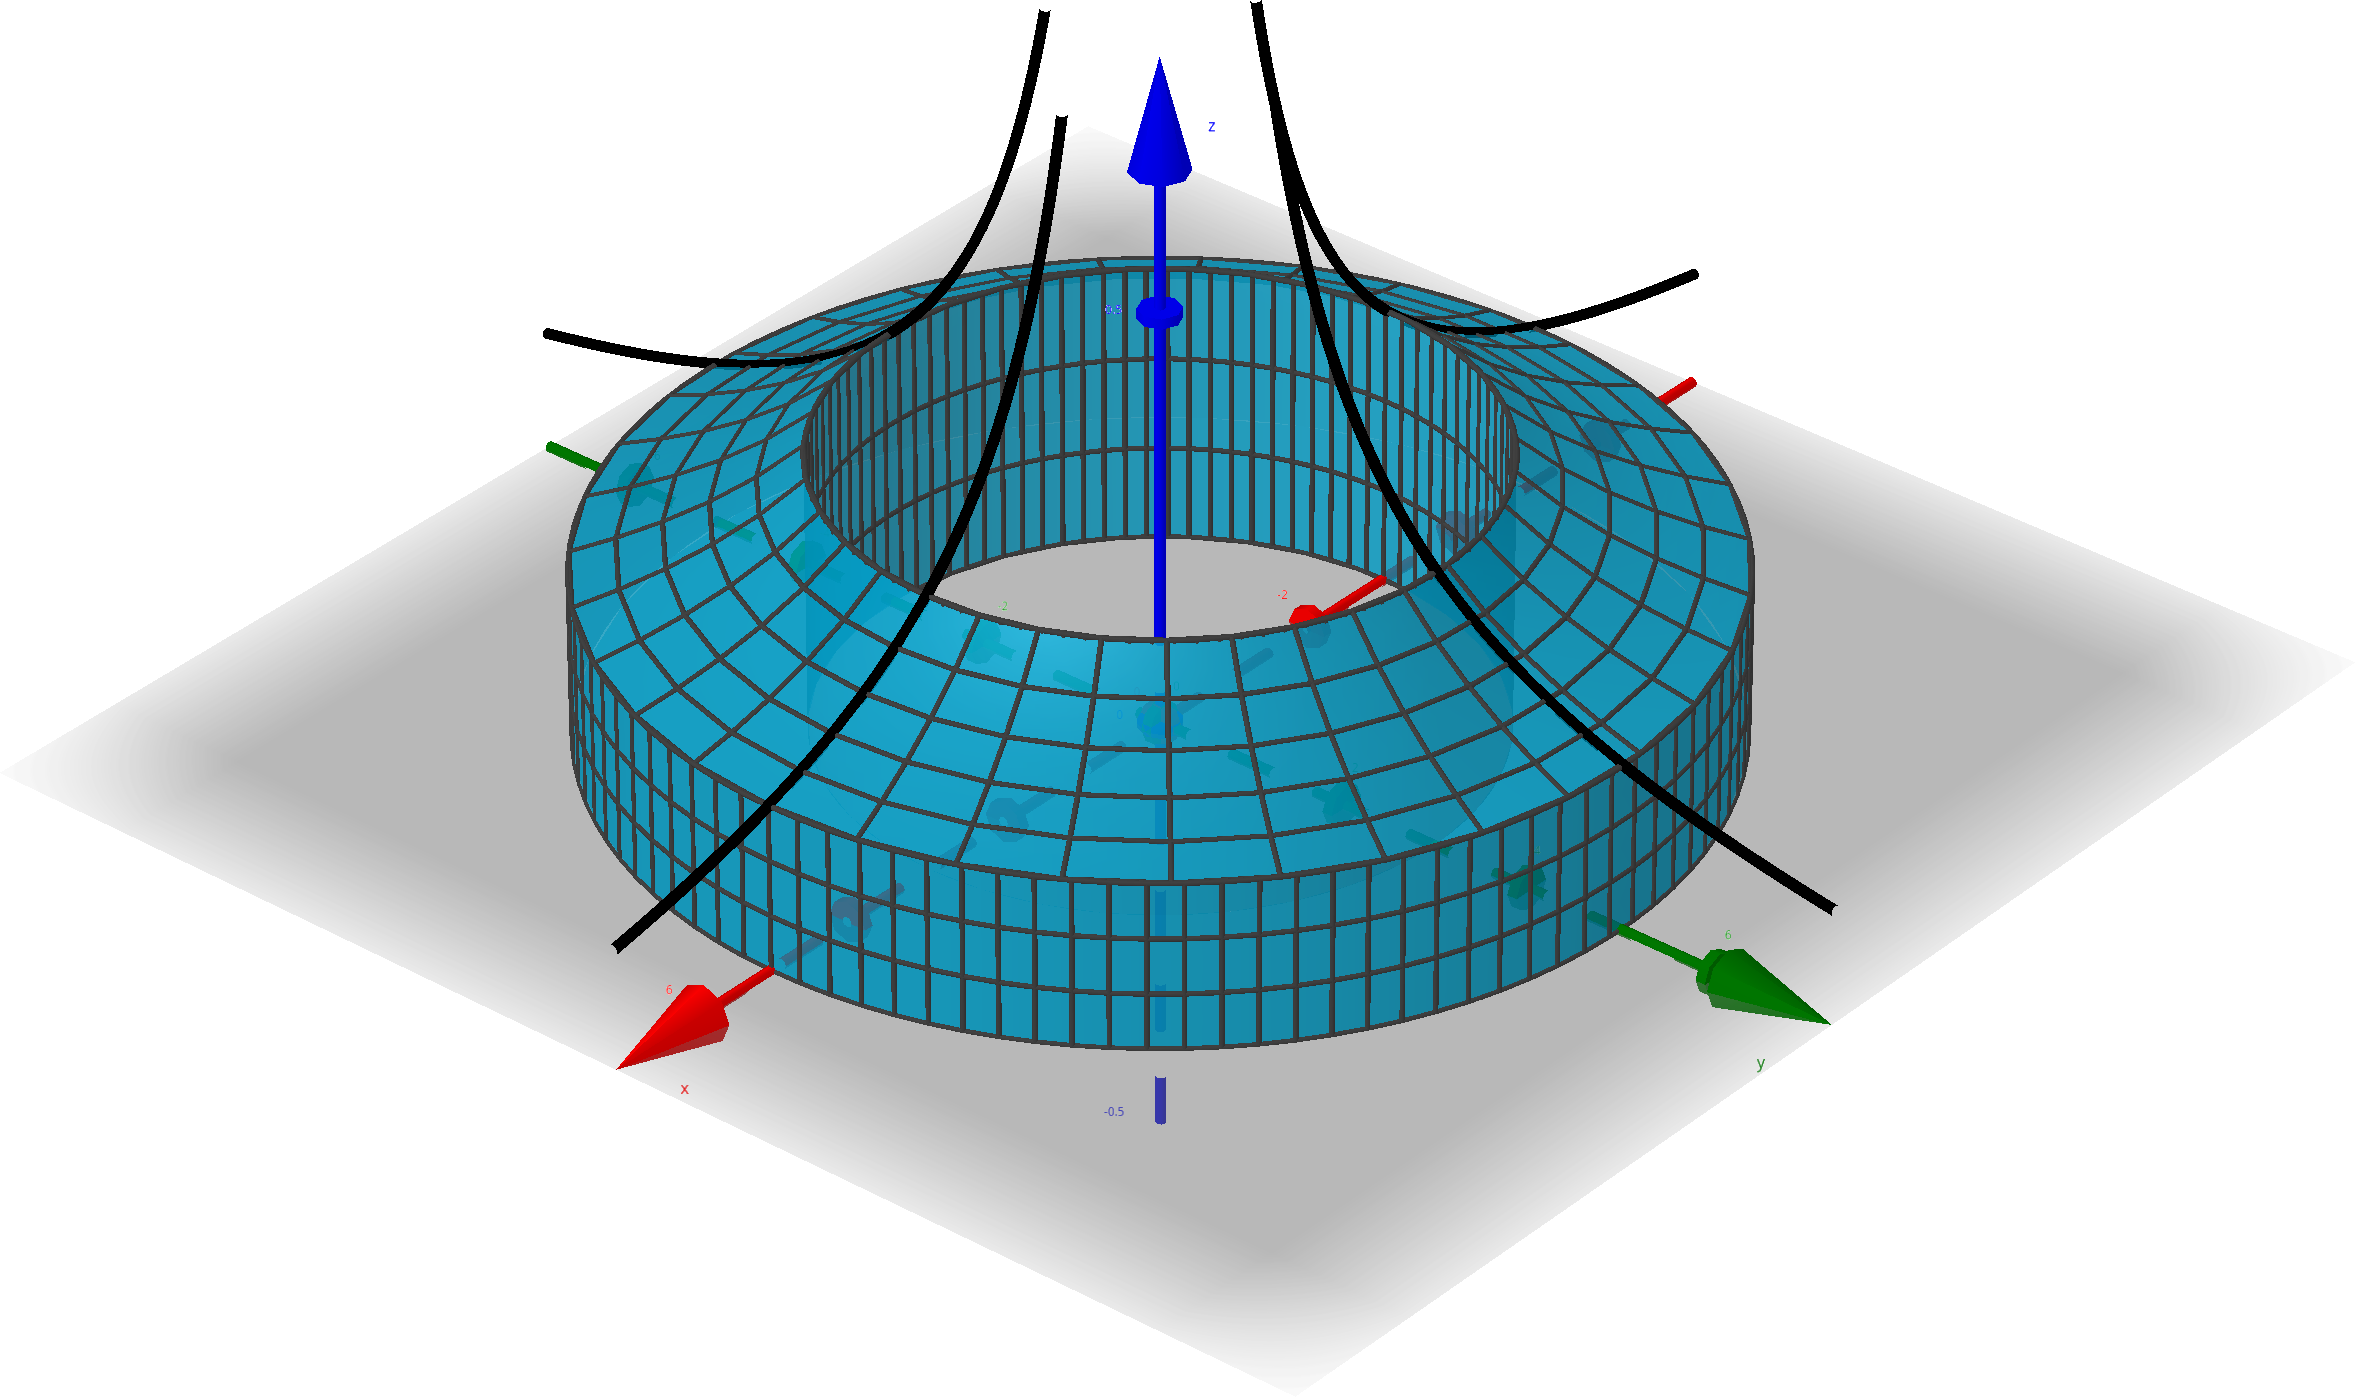
\includegraphics[width=0.5\textwidth]{img/integral-dupla.png}
\end{center}


\Exercise[title={2,5}] Calcule as integrais iteradas $\int_{0}^{1}\int_{-x}^{x}\int_{y}^{x} 6z \diff{z}\diff{y}\diff{x}$, mudando a ordem de integração, se necessário.
\Answer
\begin{align*}
    \int_{0}^{1}\int_{-x}^{x}\int_{y}^{x} 6z \diff{z}\diff{y}\diff{x}
    & = \int_{0}^{1}\int_{-x}^{x} \left[ 3z^2 \right]_{y}^{x} \diff{y}\diff{x}
      = \int_{0}^{1}\int_{-x}^{x} 3x^2 - 3y^2 \diff{y}\diff{x} \\
    & = \int_{0}^{1} \left[ 3x^2y - y^3 \right]_{-x}^{x} \diff{x}
      = \int_{0}^{1} \left[ 3x^2(x - (-x)) - (x^3 - (-x)^3) \right] \diff{x} \\
    &
      = \int_{0}^{1} 6x^3 - 2x^3 \diff{x}
      = \int_{0}^{1} 4x^3 \diff{x}
      = [x^4]_{0}^{1}
      = 1 - 0
      = 1.
\end{align*}

Portanto, \(\boxed{\int_{0}^{1} \int_{-x}^{x} \int_{y}^{x} 6z \, dz \, dy \, dx = 1}\).

\begin{center}
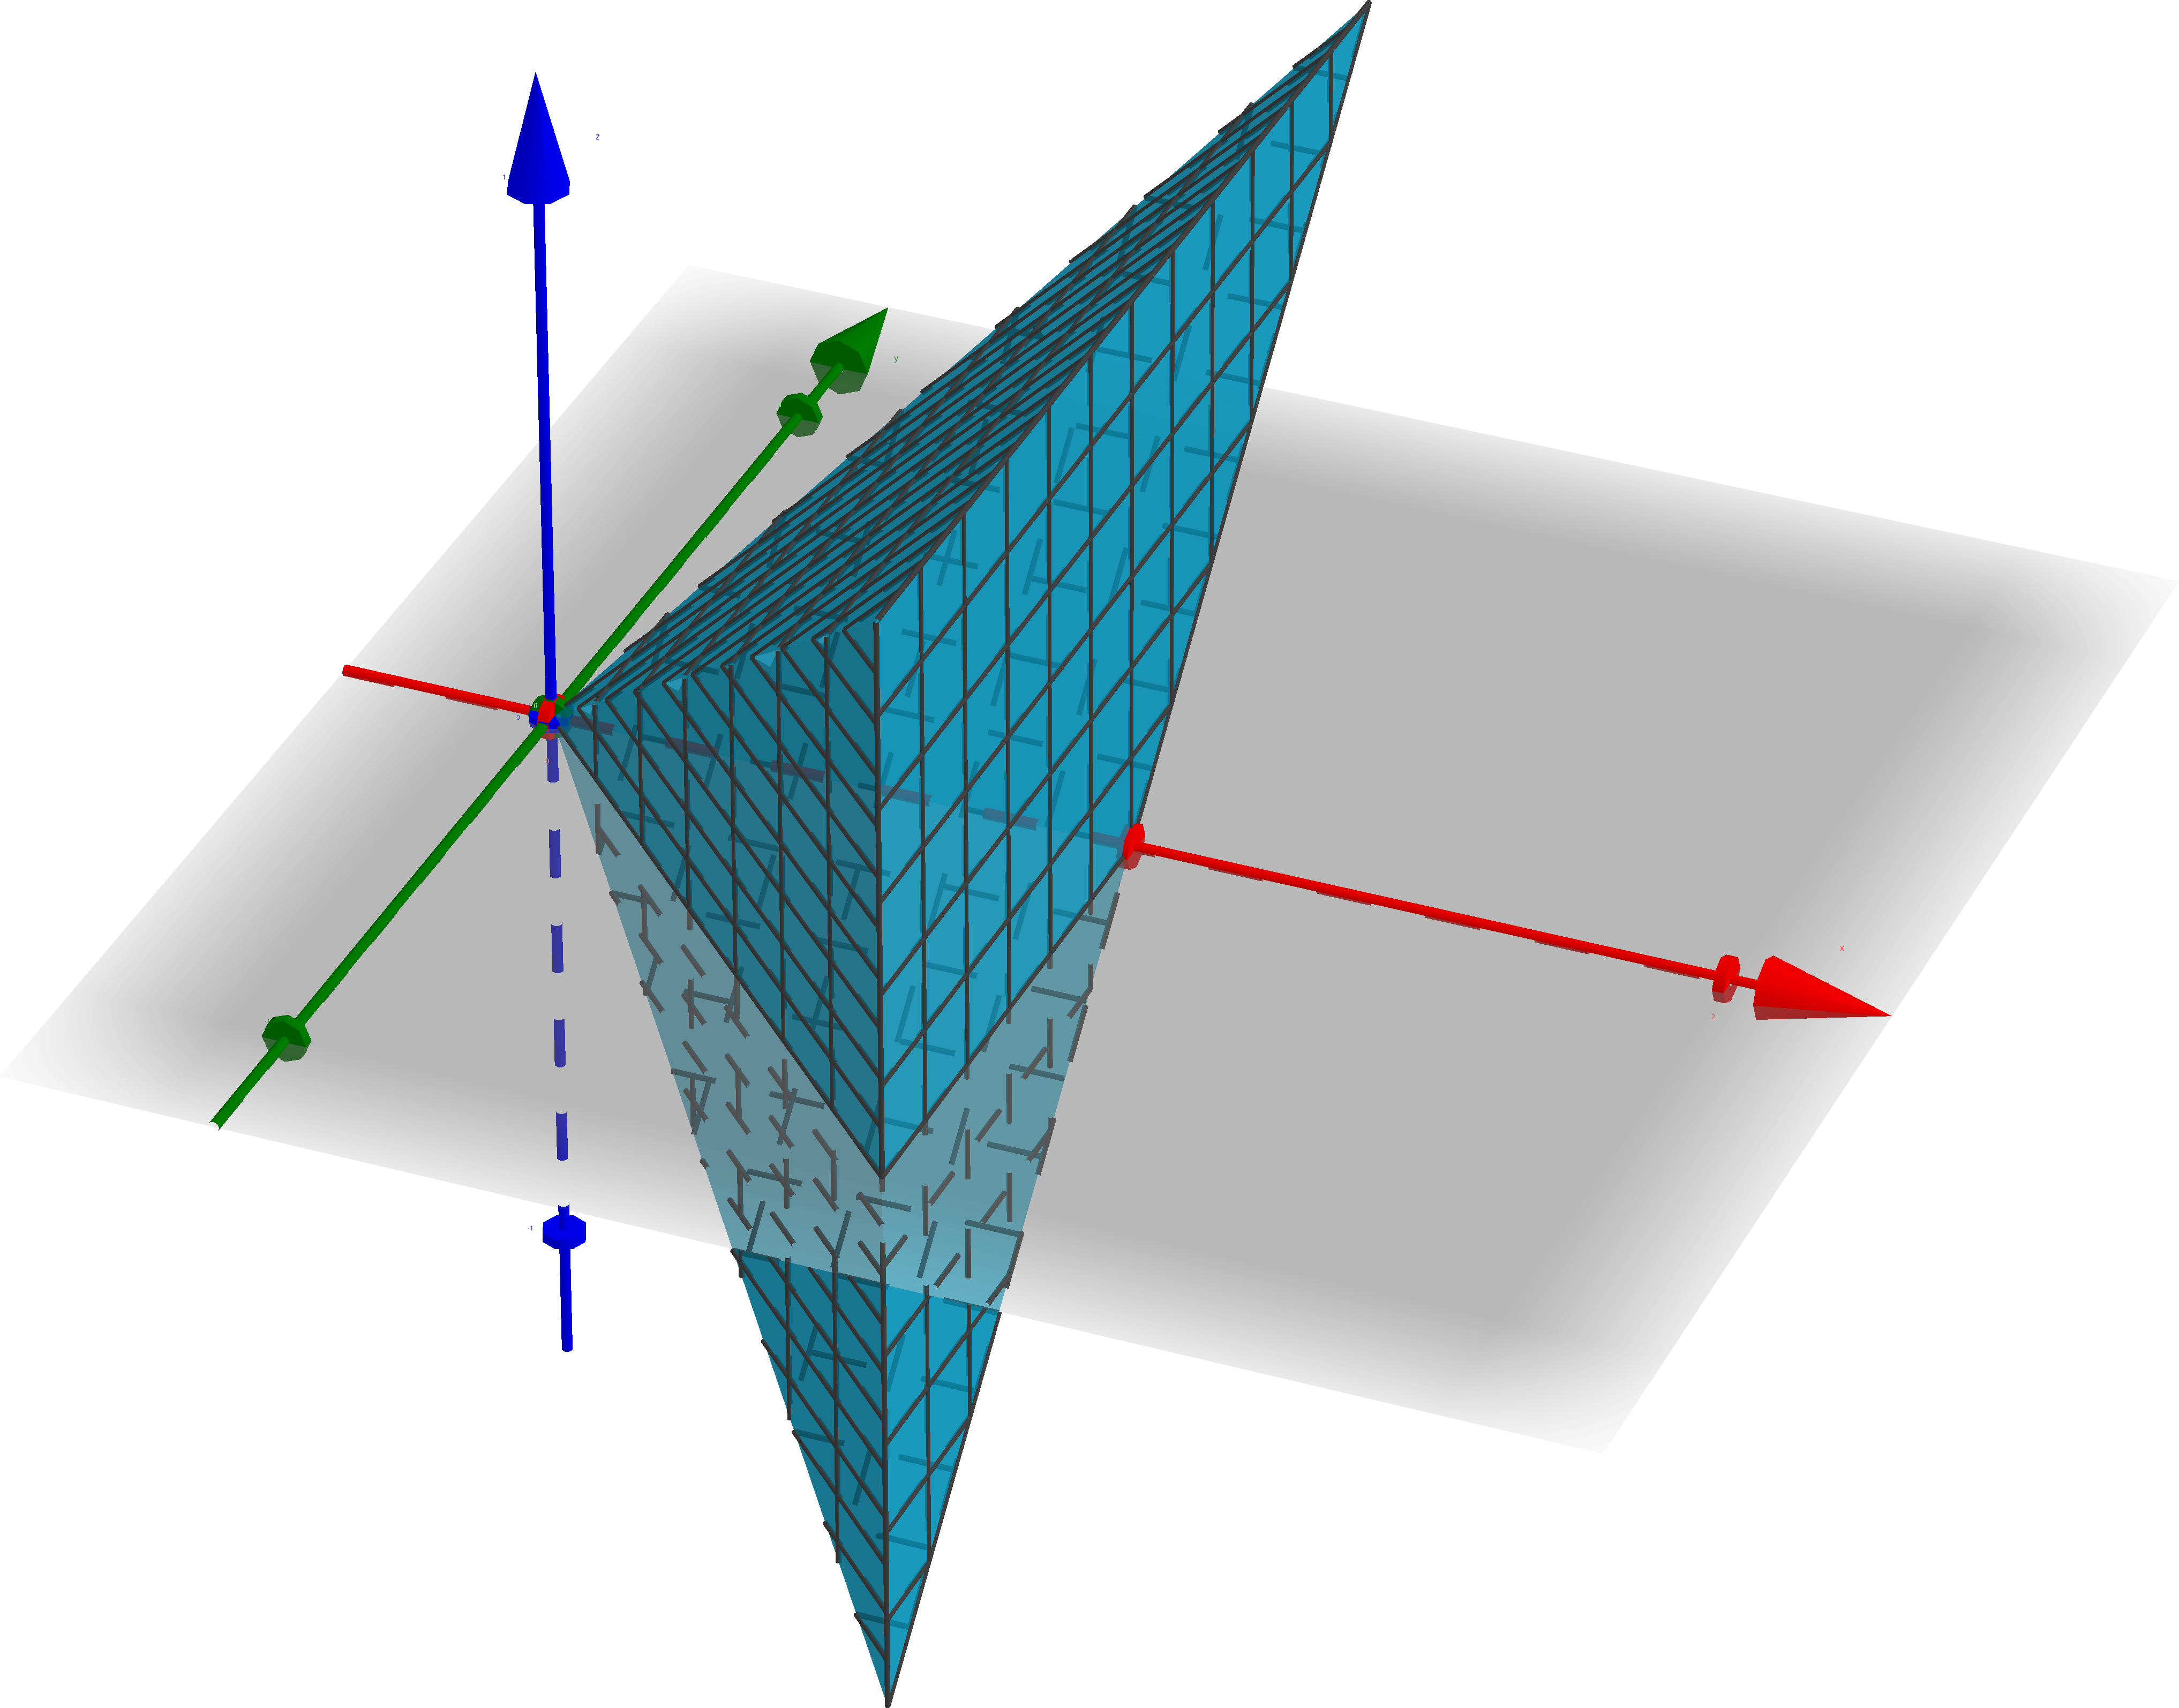
\includegraphics[width=0.5\textwidth]{img/integral-tripla-tetraedro.png}
\end{center}

\end{ExerciseList}

\vfill
\begin{center}
BOA PROVA E BOAS FÉRIAS!
\end{center}

\newpage
\restoregeometry
\section*{Respostas}
\shipoutAnswer
\end{document}
